\chapter{Structure du télescope}

\section{Projet d'origine}

La structure du télescope est imprimable à l'imprimante 3D et provient d'un projet open source entre temps disparu d'internet~:
{\href{https://blog.dagoma.fr/telescope-imprime-en-3d/}{\codeinline{text}{https://blog.dagoma.fr/telescope-imprime-en-3d/}}}

\vspace{1cm}

Voici l'allure du télescope monté. Les barres métalliques raccordant le support du miroir secondaire au reste du télescope sont des barres de camping achetées en magasin de sport.

\begin{figure}[H]
    \centering
    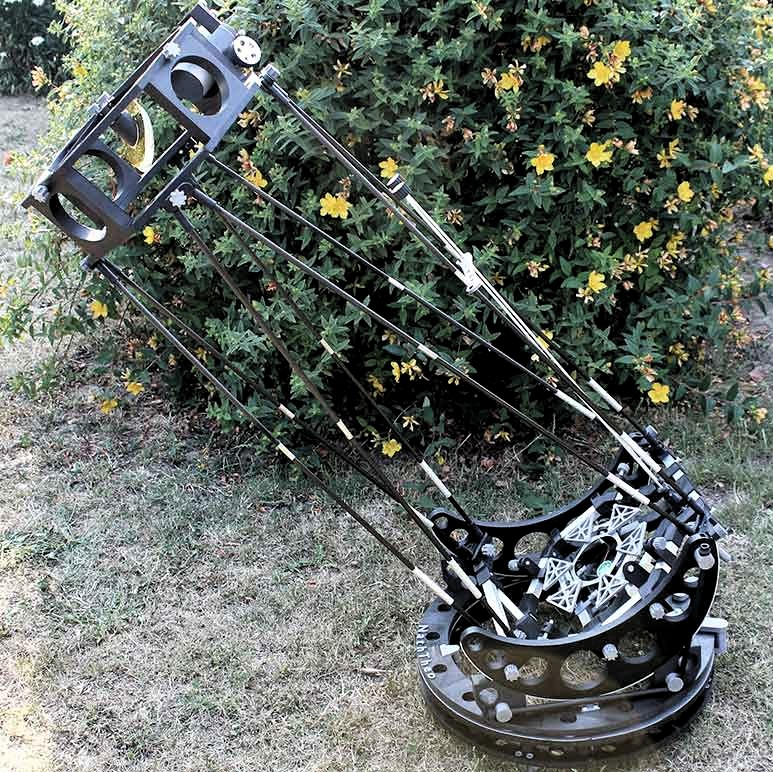
\includegraphics[width=0.5\linewidth]{\figures/photo_telescope2.jpg}
    \decoRule
    \caption[
    Photo du télescope]{
    Photo du télescope}
    \label{fig:Photo du télescope}
    \end{figure}

\begin{figure}[H]
    \centering
    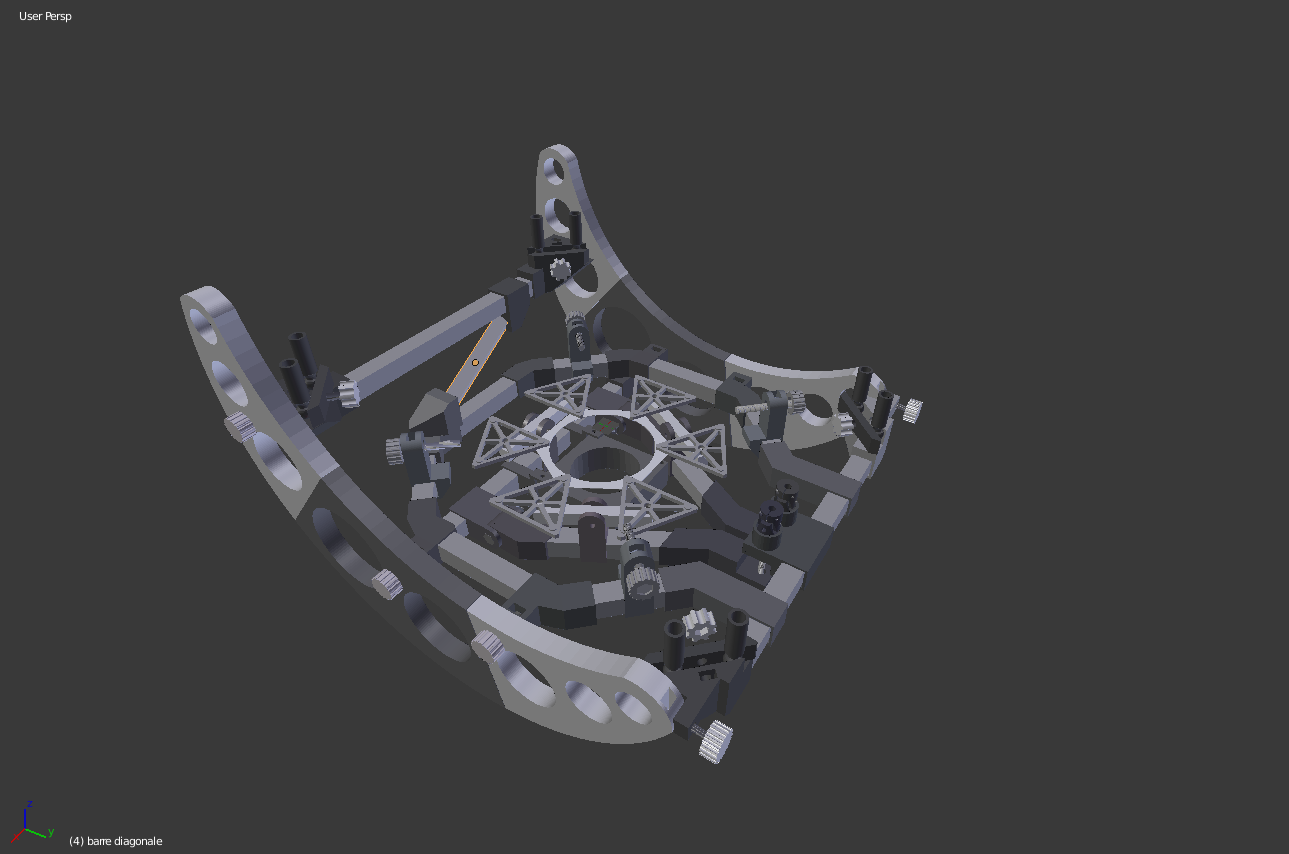
\includegraphics[width=0.49\linewidth]{\figures/blender_3.png}
    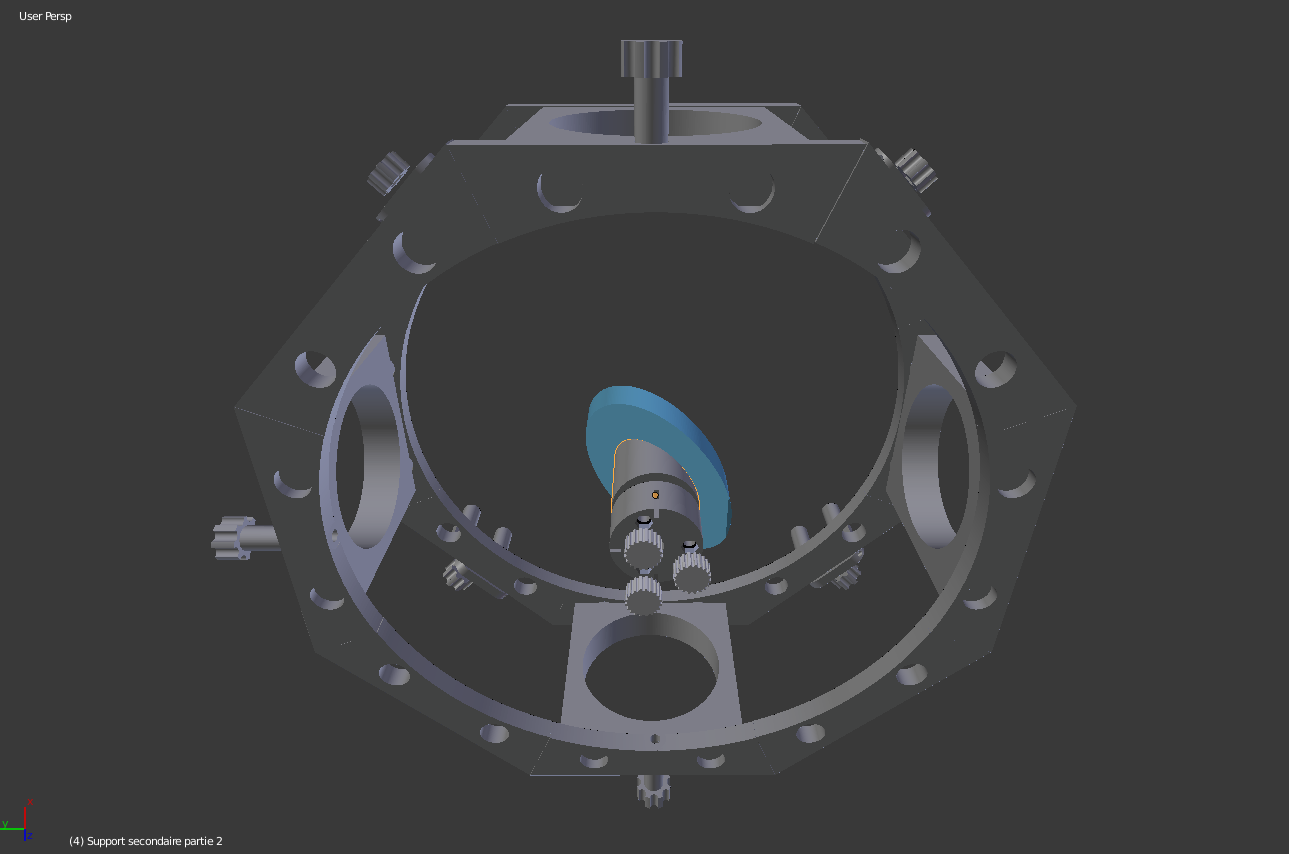
\includegraphics[width=0.49\linewidth]{\figures/blender_4.png}
    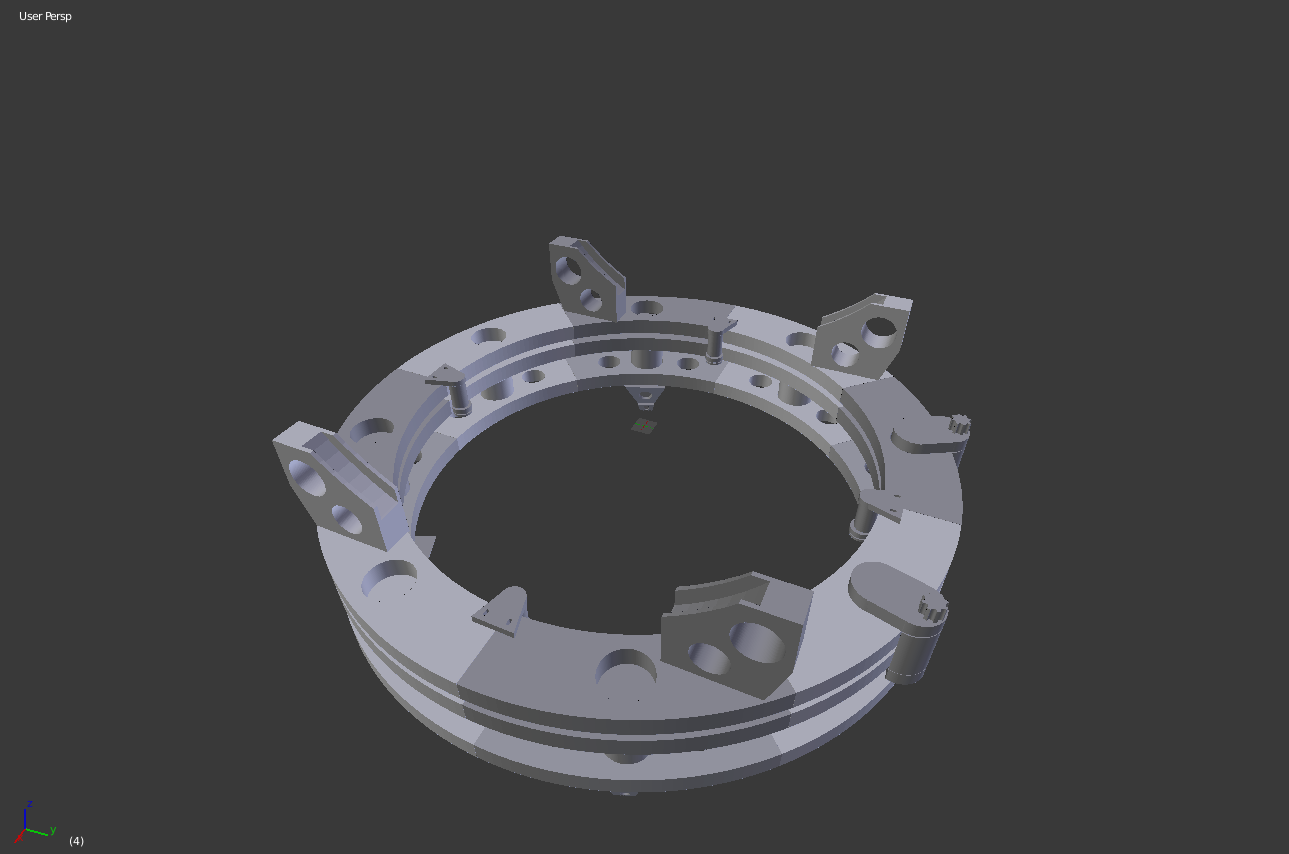
\includegraphics[width=0.49\linewidth]{\figures/blender_5.png}
    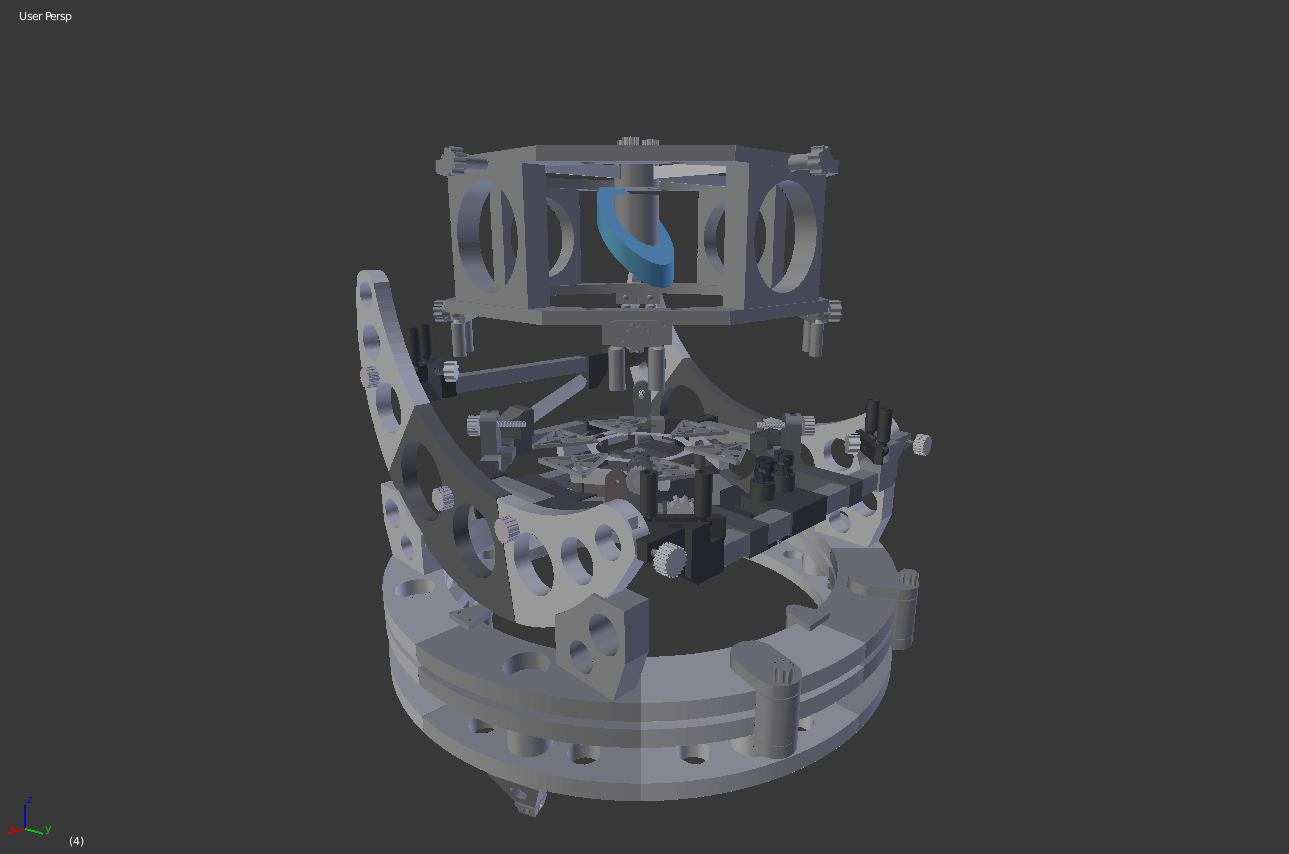
\includegraphics[width=0.49\linewidth]{\figures/blender_6.png}
    \decoRule
    \caption[
    Aperçu des fichiers de production du télescope]{
    Aperçu des fichiers de production du télescope}
    \label{fig:Aperçu des fichiers de production du télescope}
    \end{figure}

\section{Étude de la robotisation du télescope}

Ci-dessous quelques schémas représentant les modifications, telles qu'imaginées, à apporter à la structure du télescope pour l'automatiser.

\vspace{1cm}

Le socle, immobile, sera doté d'une courroie ainsi que d'un cran permettant d'activer le capteur de position. Le système électronique sera solidaire du support du miroir primaire, mobile, à l'étage supérieur. Un moteur doté d'une roue crantée fixé sur la plateforme tournante permettra de la mettre en mouvement par rapport au socle.

\begin{figure}[H]
    \centering
    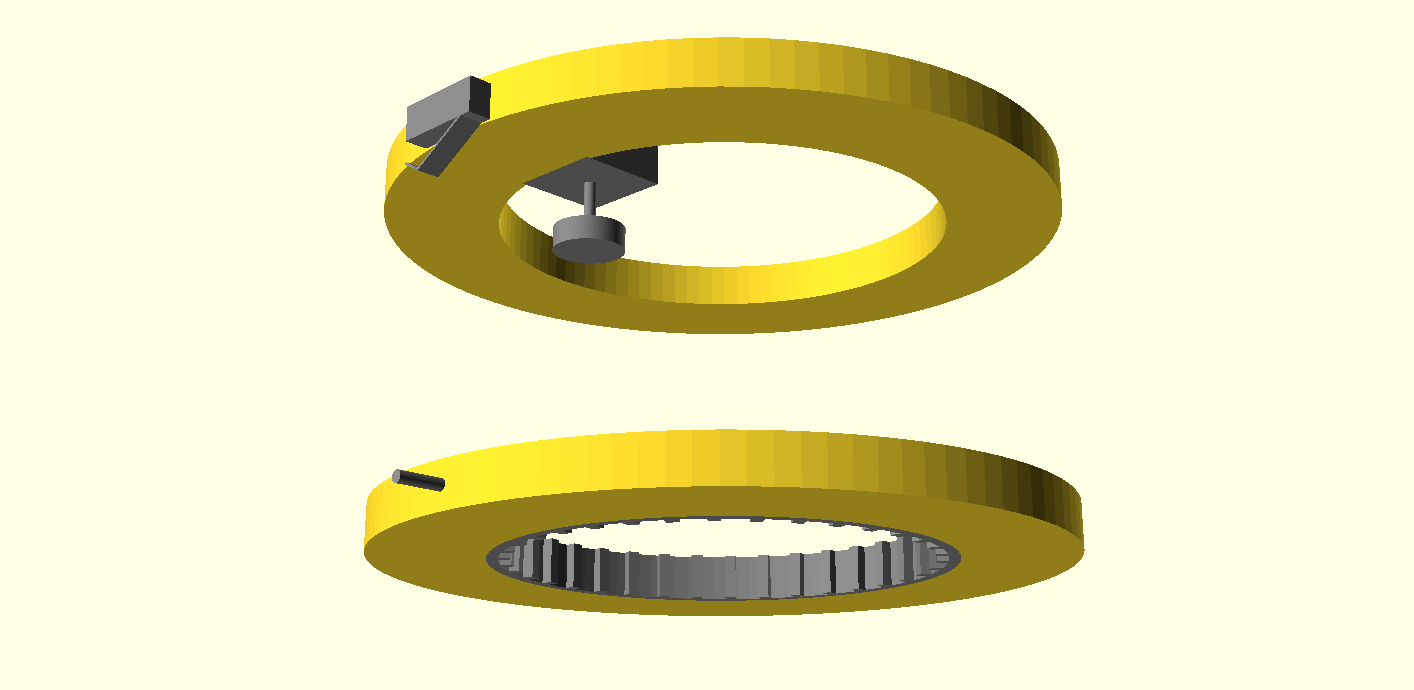
\includegraphics[width=0.9\linewidth]{\figures/OpenSCAD/azim.png}
    \decoRule
    \caption[
    Schéma du mécanisme permettant un mouvement azimutal]{
    Schéma du mécanisme permettant un mouvement azimutal}
    \label{fig:Schéma du mécanisme permettant un mouvement azimutal}
    \end{figure}

\vspace{1cm}

Pour le mouvement d'élévation, un système de tringlerie et de courroie a été imaginé pour mouvoir le support du miroir primaire par rapport à la plateforme tournante. Deux capteurs de position judicieusement placés permettront de détecter lorsque le mouvement atteint l'un de ses maximums.

\begin{figure}[H]
    \centering
    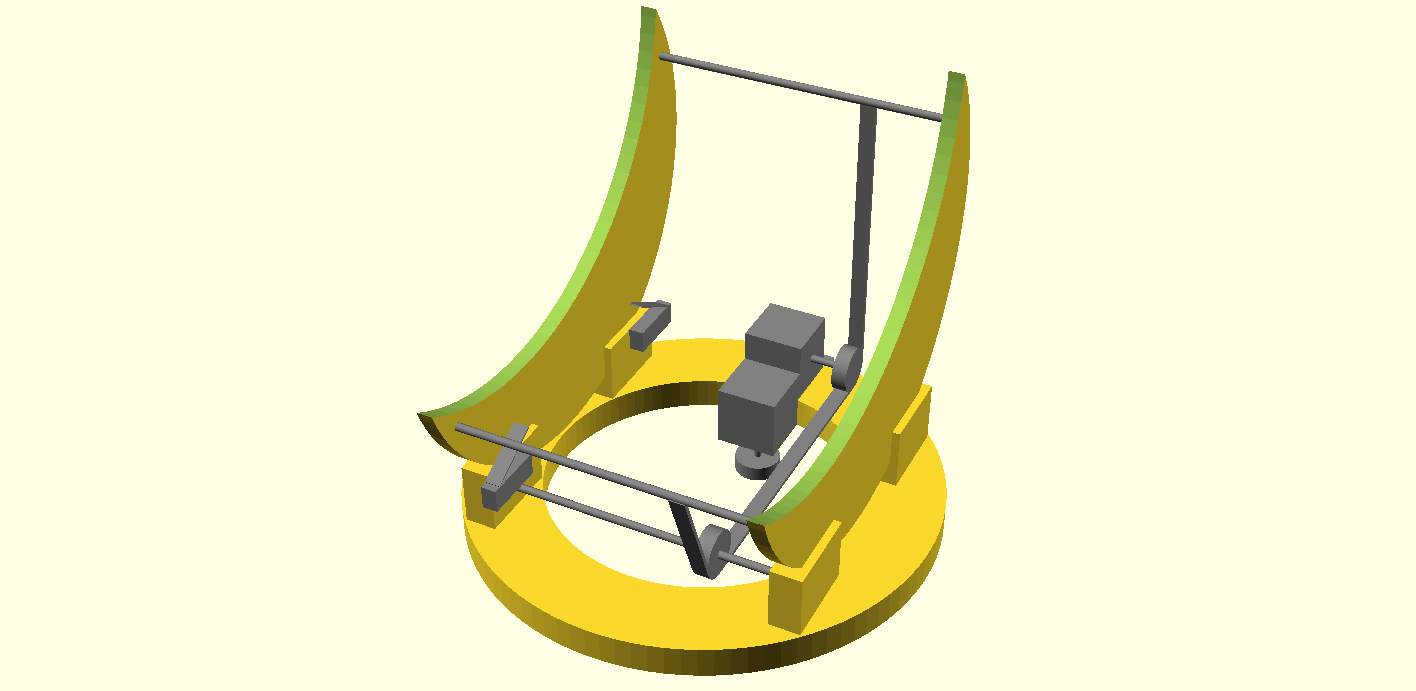
\includegraphics[width=0.9\linewidth]{\figures/OpenSCAD/elev3.png}
    \decoRule
    \caption[
    Schéma du mécanisme permettant un mouvement d'élévation]{
    Schéma du mécanisme permettant un mouvement d'élévation}
    \label{fig:Schéma du mécanisme permettant un mouvement d'élévation}
    \end{figure}

\vspace{1cm}

Quant au zoom, il faudra créer un ensemble de pièces pour maintenir le zoom lui même, la caméra (non représentée), le moteur permettant d'actionner le zoom, les capteurs de positions extrêmes, ainsi qu'un système permettant de régler finement la position de l'oculaire et de la caméra.

Un cran pour activer les capteurs de positions extrêmes pourrait être fixé à l'oculaire avec un collier de serrage par exemple.

\begin{figure}[H]
    \centering
    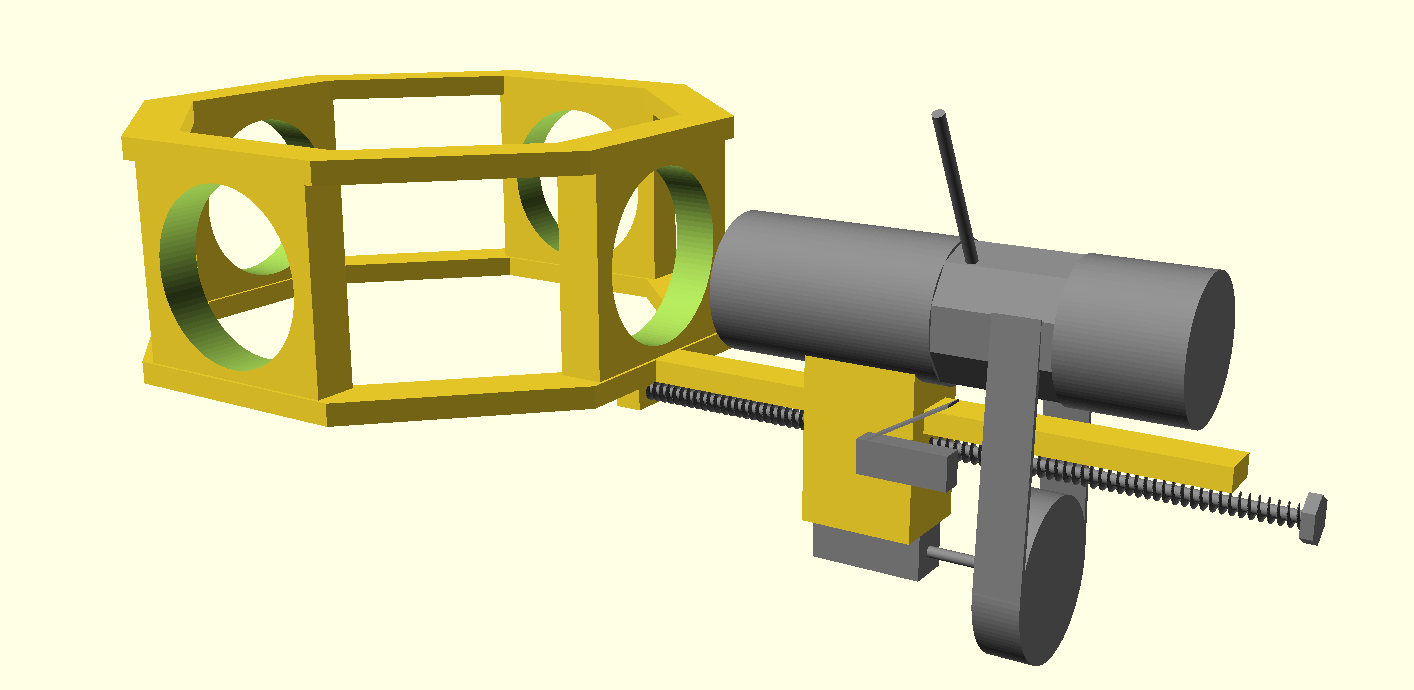
\includegraphics[width=0.9\linewidth]{\figures/OpenSCAD/zoom.png}
    \decoRule
    \caption[
    Schéma du mécanisme permettant un mouvement du zoom]{
    Schéma du mécanisme permettant un mouvement du zoom}
    \label{fig:Schéma du mécanisme permettant un mouvement du zoom}
    \end{figure}

\section{État actuel de la structure}

Pour l'instant nous avons imprimé toutes les pièces fournies par le projet original. Certaines ont subi une détérioration de la qualité lors de l'impression pour une raison mal connue et demeurent à réimprimer. Le Socle, la plateforme tournante et le support du miroir secondaire ont été montés. Aucune modification de la structure en vue d'y intégrer le système électronique n'a été faite.

\begin{figure}[H]
    \centering
    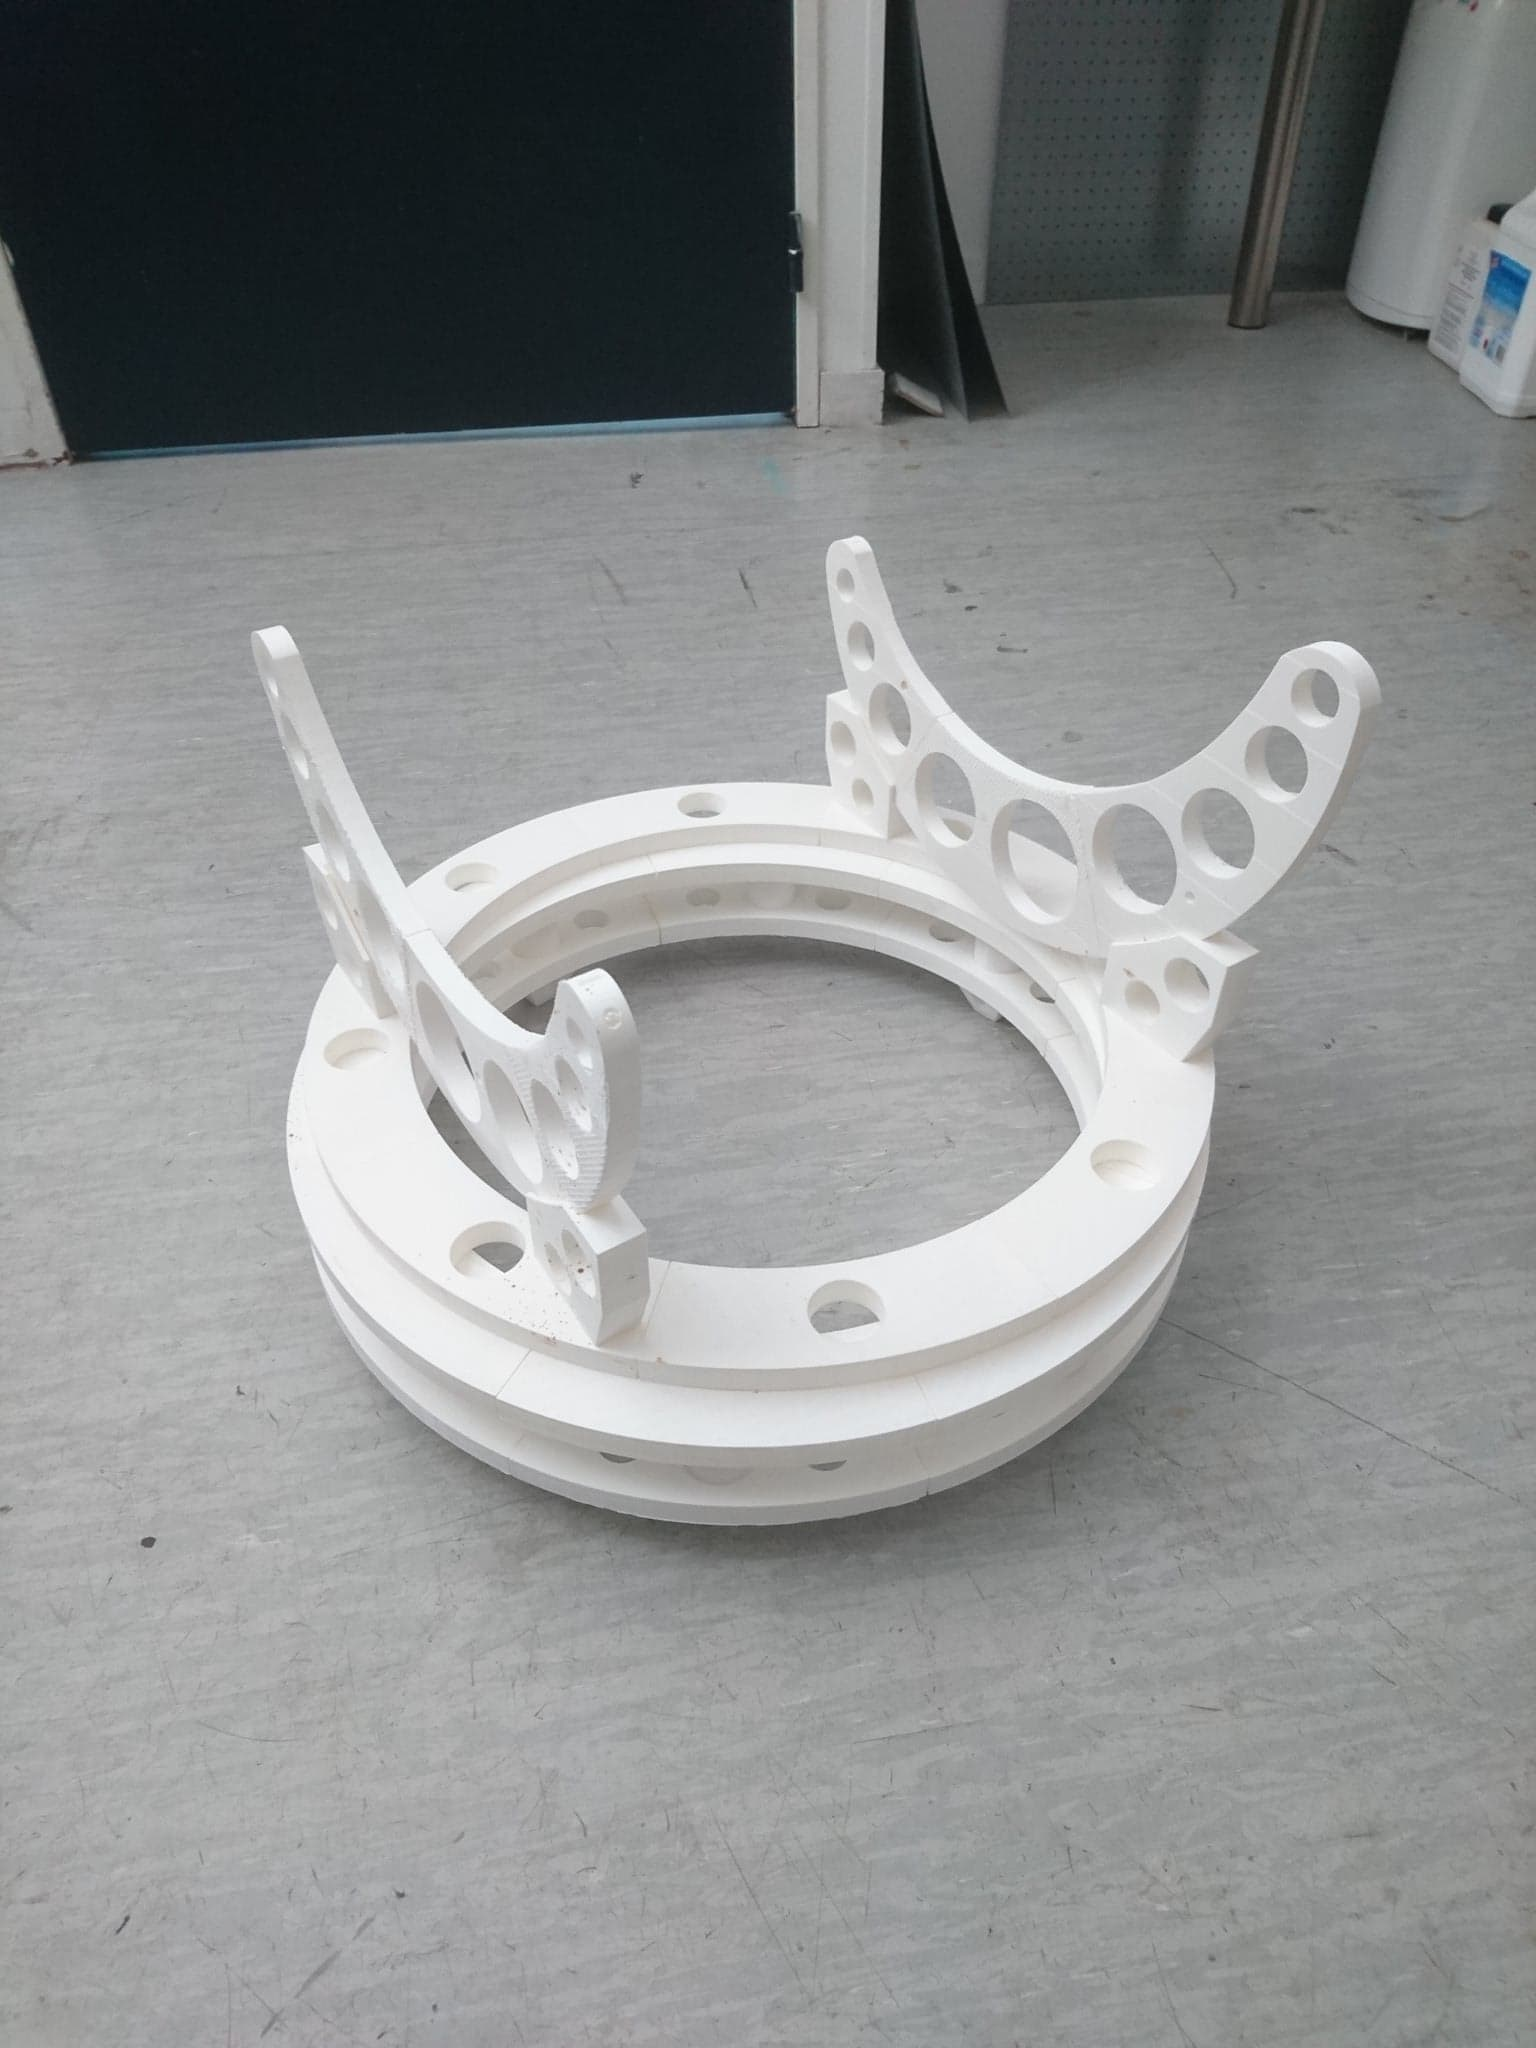
\includegraphics[width=0.3\linewidth]{\figures/photo_structure1.jpg}
    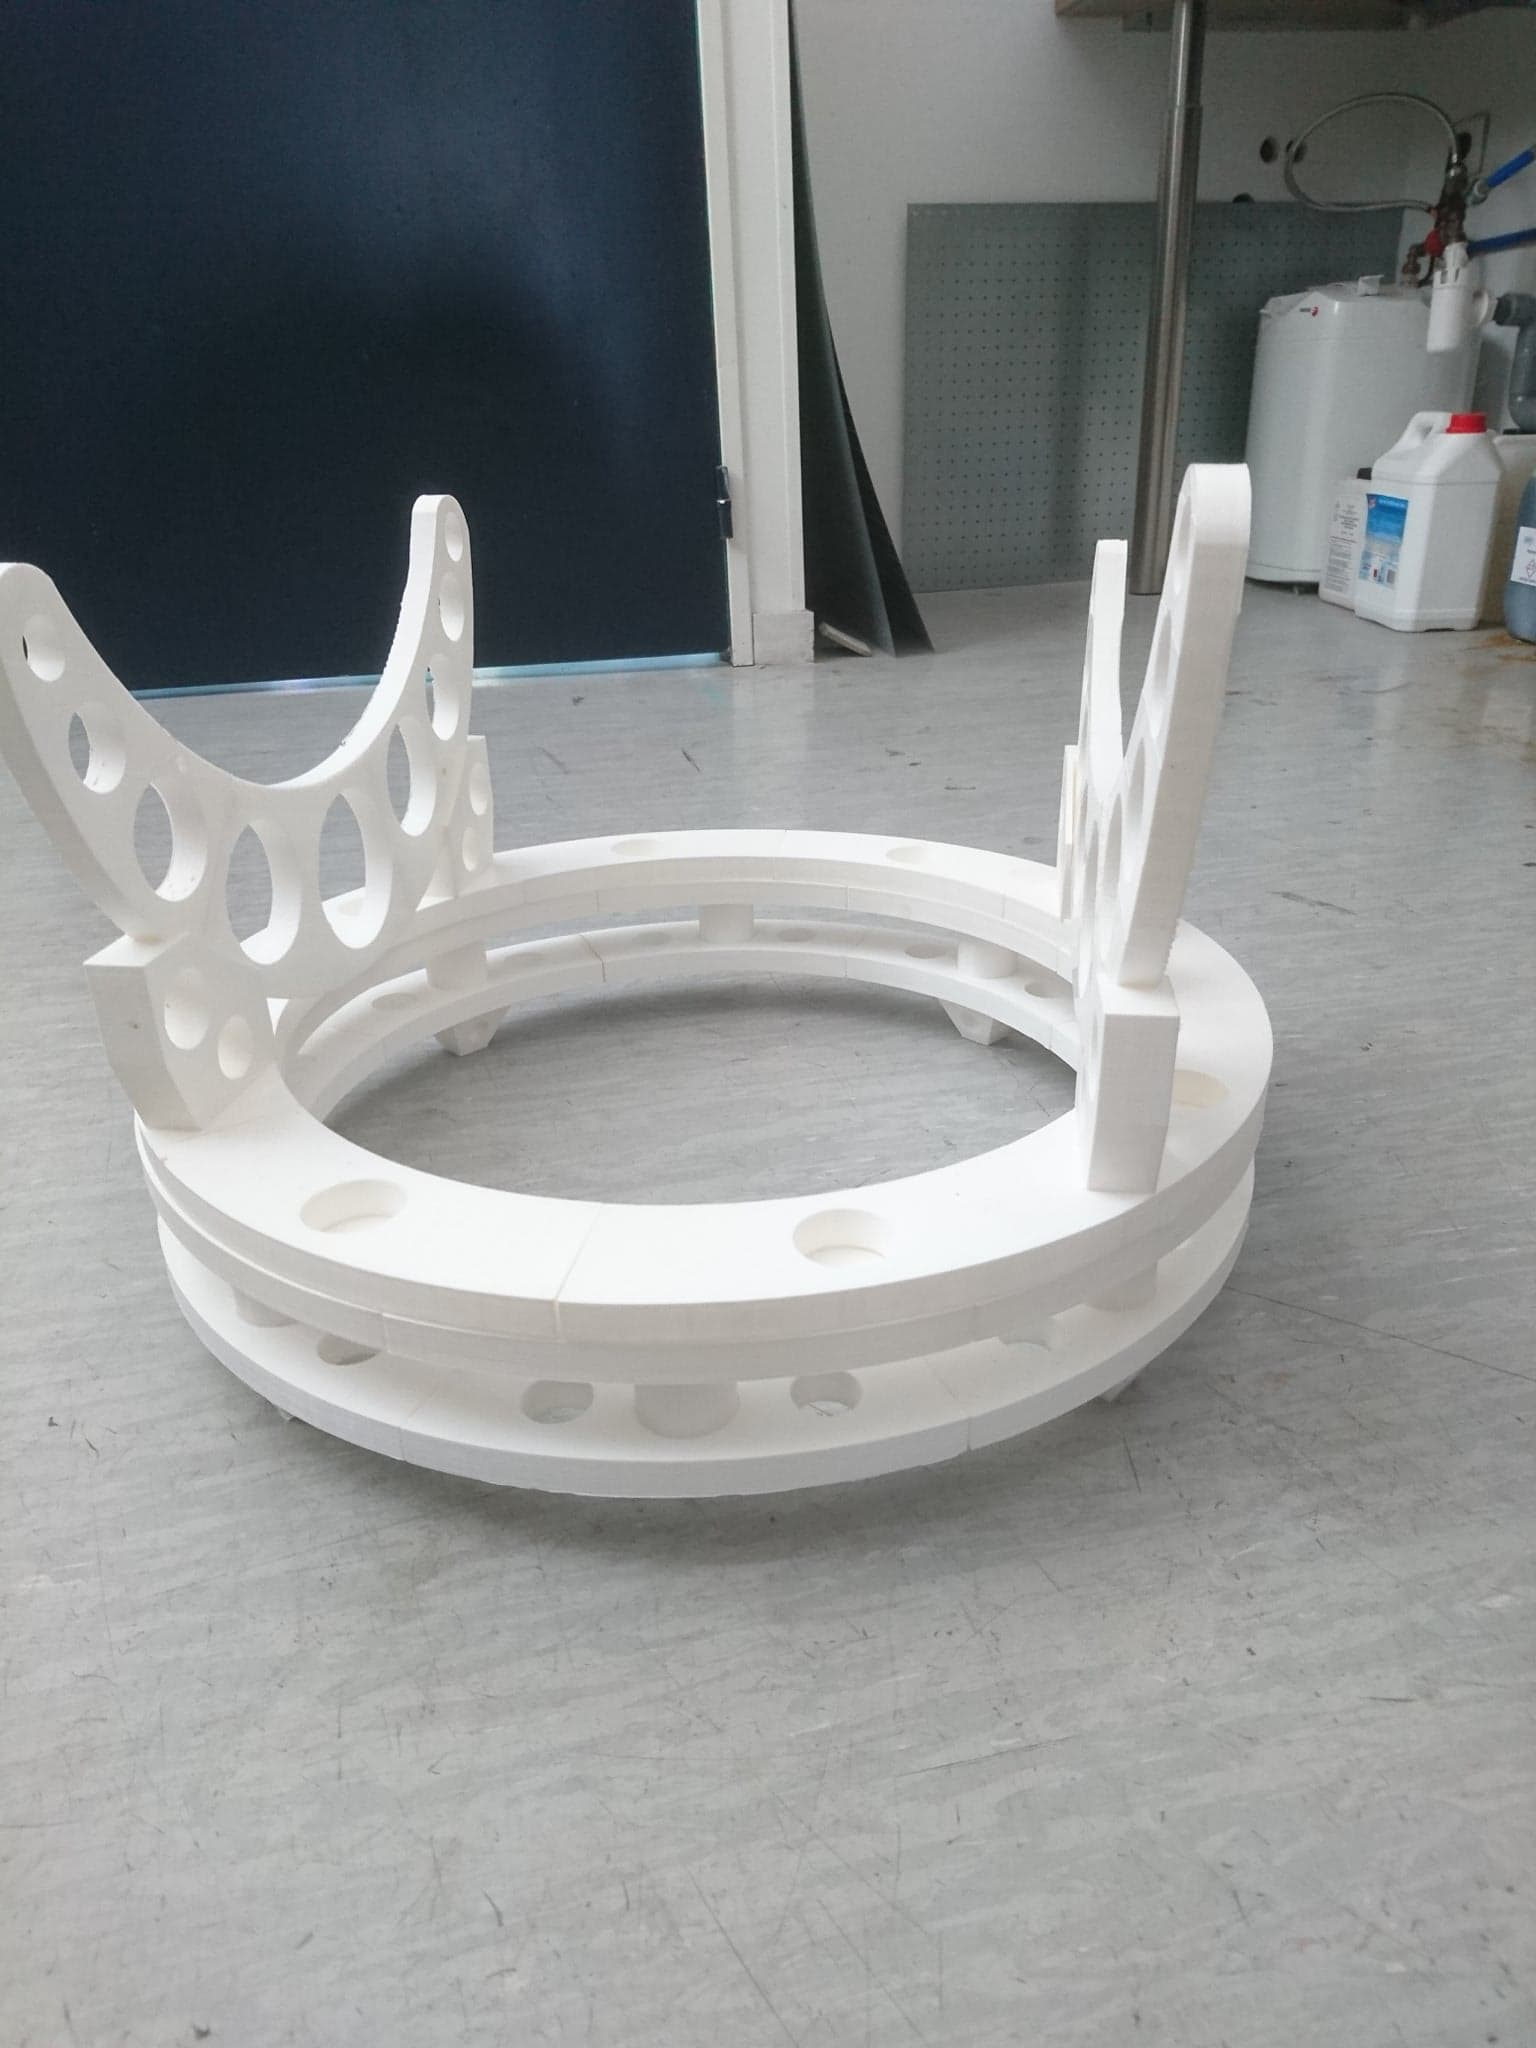
\includegraphics[width=0.3\linewidth]{\figures/photo_structure2.jpg}
    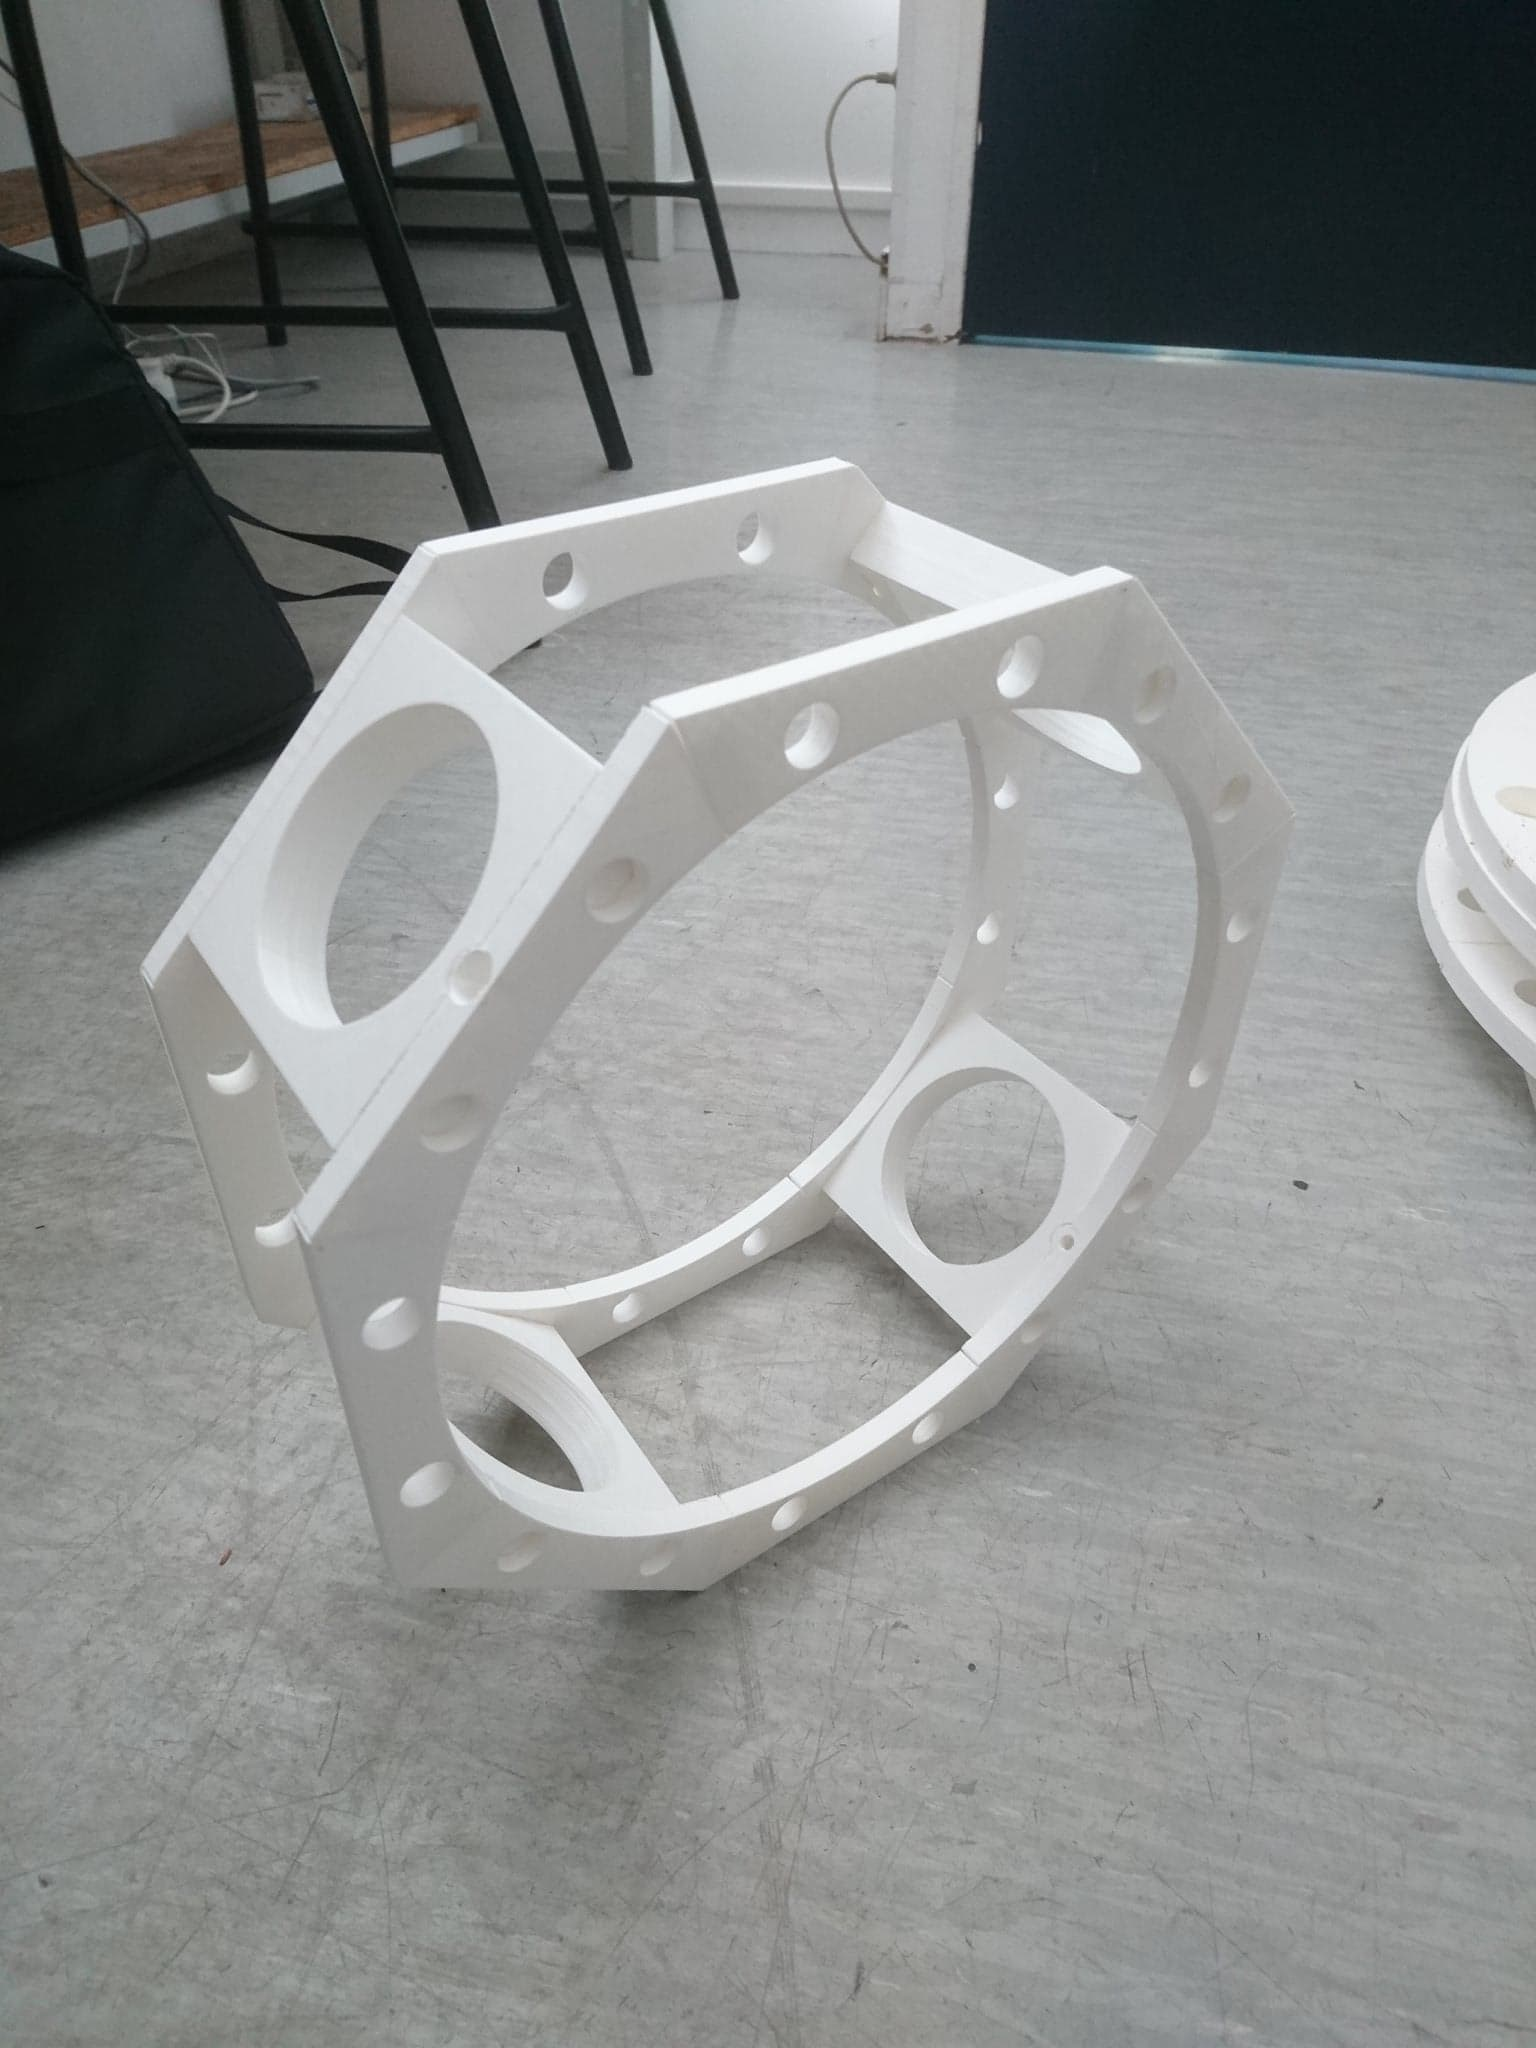
\includegraphics[width=0.3\linewidth]{\figures/photo_structure3.jpg}
    \decoRule
    \caption[
    Photos des parties montées du télescope]{
    Photos des parties montées du télescope}
    \label{fig:Photos des parties montées du télescope}
    \end{figure}

